\section{System Evaluation}

TODO: summary for this chapter

\subsection{Success Criterias}

  \subsubsection{Model Evaluation}

  Malicious player detection is a classification problem. 
  One can generate random data and test the performance of PRM through accuracy and recall, even ROC curve \cite{hanley1982meaning}.

  The click behavior has been researched for years and address by FFitts Law \cite{bi2013ffitts}.
  It modeled and proved the distribution of click behavior for a certain click goal point is a normal distribution.
  Thus, with probablistic view, the top left corner of ROI exists, then the user click selection 
  for this point should follows normal distribution, as shown in figure \ref{fig:evaluation}.

  \begin{figure}[htp]
  \centering
  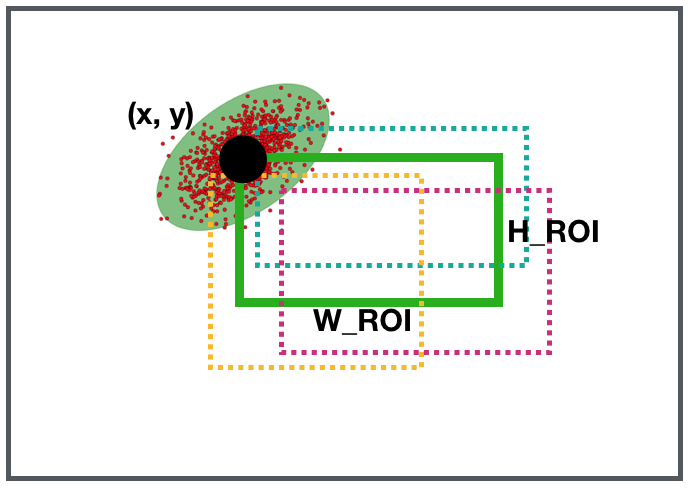
\includegraphics[width=0.5\columnwidth]{figures/evaluation}
  \caption{Data Simulation}
  \label{fig:evaluation}
  \end{figure}

  Therefore, to generate ROIs, let $(x, y)$ is the player ROI start point,  $(H_{ROI}$, $W_{ROI})$ is the height
  and width pair of this ROI, then we generate the random dataset for these variables by a given
  parameter $\delta$: $(x, y) \sim (x+N(0, \delta), y+N(0, \delta)), (H_{ROI}, W_{ROI}) \sim (H_{ROI}+N(0, \delta), W_{ROI}+N(0, \delta))$.
  To generate tags, we propose randomly pick random number of tags.

  Then one can perform this random dataset on our system to evaluate the classification accuracy and recall rate to
  evaluate the overall performance of this system, which gives the theoretical evaluation results.

  \subsubsection{Issues on Social and Ethical Aspects}

  TODO: More discussion on the social ethical aspects

\subsection{Limitations of the System}

  \subsubsection{Evaluation Outdate}

  A limitation occurs in our social network based model is each disaster level evaluation get invalid 
  if the region image outdate. 
  We assume the satellite monitors a region and take picutre between intervals. However, our evaluation
  model only calculate the disaster level at a unique moment, which means the disaster level need 
  transvaluation when a new image come out.
  If our player are not enough so that the region images always have to wait new evaluation, then the
  disaster level will never be calculated.

  A possible solution is to consider the region disaster level history as a time series. Then we can apply
  some prediction method for it. For instance, we have time series: $(t_1, t_2, t_3, ..., t_n)$
  and its corresponding disaster level: $(DL_1, DL_2, DL_3, ..., DL_n)$.
  Then we can use these time series to predict the disaster level at time $t_{n+1}$.

  At the same time, we also have the historical data of trust value of a player. We can also
  use time series prediction to predict the players trust value. But in all of these, the time series
  of disaster level is not stationary but the time series of trust value is stationary.

  \subsubsection{Information Loss}
  We cut big region images into small fragement areas to prevent leakage of data. 
  But this method will cause some information loss problem if some important ROIs are 
  located at the intersection of two dividing lines.
  A possible solution for this limitation is to cut the big image with a random distance 
  between two adjacency dividing lines, as shown in figure \ref{fig:information_loss}.

  \begin{figure}[htp]
  \centering
  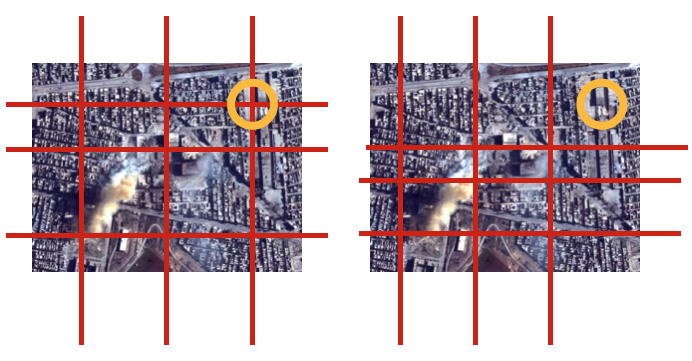
\includegraphics[width=0.5\columnwidth]{figures/information_loss}
  \caption{Information Loss Solution (TODO: Modify Image)}
  \label{fig:information_loss}
  \end{figure}

  \subsubsection{Gameplay and Playability}
  The HC system collect satellite photos of disaster areas. But even if in the disaster areas, 
  not every part of the areas has disaster. Most parts of the earth are lake, forest, 
  desert and so on, which means the users may meet the situation that there is no available 
  ROI in several continuous rounds. Obviously, it will decrease the playability and enjoyment of the game.
  Our system is just a very simple tagging game at present, users can not get enough enjoyment they want in it. 
  And it is too reliant on the unpaid volunteers to donate their time to contribute information. 
  We should make the system more interesting and appealing in the future work.
